\documentclass[a4paper,11pt]{book}
%\documentclass[a4paper,twoside,11pt,titlepage]{book}
\usepackage{listings}
\usepackage[utf8]{inputenc}
\usepackage[spanish]{babel}
\usepackage{subfig}

% \usepackage[style=list, number=none]{glossary} %
%\usepackage{titlesec}
%\usepackage{pailatino}

\decimalpoint
\usepackage{dcolumn}
\newcolumntype{.}{D{.}{\esperiod}{-1}}
\makeatletter
\addto\shorthandsspanish{\let\esperiod\es@period@code}
\makeatother


%\usepackage[chapter]{algorithm}
\RequirePackage{verbatim}
%\RequirePackage[Glenn]{fncychap}
\usepackage{fancyhdr}
\usepackage{graphicx}
\usepackage{afterpage}
\usepackage{amsmath}
\usepackage{amsfonts}
\usepackage{longtable}
\usepackage{minted}

\usepackage[pdfborder={000}]{hyperref} %referencia

% ********************************************************************
% Re-usable information
% ********************************************************************
\newcommand{\myTitle}{Groebner-Robotics \xspace}
\newcommand{\myDegree}{Doble Grado en Ingeniería Informática y Matemáticas \xspace}
\newcommand{\myName}{Antonio Solís Izquierdo \xspace}
\newcommand{\myProf}{Pedro A. García-Sánchez \xspace}
\newcommand{\myFaculty}{Facultad de Ciencias \xspace}
\newcommand{\myFacultyShort}{F. Ciencias \xspace}
\newcommand{\myDepartment}{Departamento de ... \xspace}
\newcommand{\myUni}{\protect{Universidad de Granada} \xspace}
\newcommand{\myLocation}{Granada \xspace}
\newcommand{\myTime}{\today \xspace}
\newcommand{\myVersion}{Version 0.1 \xspace}


\hypersetup{
pdfauthor = {\myName (asolisi (en) ugr (punto) es)},
pdftitle = {\myTitle},
pdfsubject = {},
pdfkeywords = {palabraclave1, palabraclave2, palabraclave3, ...},
pdfcreator = {LaTeX con el paquete ....},
pdfproducer = {pdflatex}
}

\hyphenation{}


%\usepackage{doxygen/doxygen}
%\usepackage{pdfpages}
\usepackage{url}
\usepackage{colortbl,longtable}
\usepackage[stable]{footmisc}
%\usepackage{index}

%\makeindex
%\usepackage[style=long, cols=2,border=plain,toc=true,number=none]{glossary}
% \makeglossary

% Definición de comandos que me son tiles:
%\renewcommand{\indexname}{Índice alfabético}
%\renewcommand{\glossaryname}{Glosario}

\pagestyle{fancy}
\fancyhf{}
\fancyhead[LO]{\leftmark}
\fancyhead[RE]{\rightmark}
\fancyhead[RO,LE]{\textbf{\thepage}}
\renewcommand{\chaptermark}[1]{\markboth{\textbf{#1}}{}}
\renewcommand{\sectionmark}[1]{\markright{\textbf{\thesection. #1}}}

\setlength{\headheight}{1.5\headheight}

\newcommand{\HRule}{\rule{\linewidth}{0.5mm}}
%Definimos los tipos teorema, ejemplo y definición podremos usar estos tipos
%simplemente poniendo \begin{teorema} \end{teorema} ...
\newtheorem{teorema}{Teorema}[chapter]
\newtheorem{ejemplo}{Ejemplo}[chapter]
\newtheorem{definicion}{Definición}[chapter]

\definecolor{gray97}{gray}{.97}
\definecolor{gray75}{gray}{.75}
\definecolor{gray45}{gray}{.45}
\definecolor{gray30}{gray}{.94}

\lstset{ frame=Ltb,
     framerule=0.5pt,
     aboveskip=0.5cm,
     framextopmargin=3pt,
     framexbottommargin=3pt,
     framexleftmargin=0.1cm,
     framesep=0pt,
     rulesep=.4pt,
     backgroundcolor=\color{gray97},
     rulesepcolor=\color{black},
     %
     stringstyle=\ttfamily,
     showstringspaces = false,
     basicstyle=\scriptsize\ttfamily,
     commentstyle=\color{gray45},
     keywordstyle=\bfseries,
     %
     numbers=left,
     numbersep=6pt,
     numberstyle=\tiny,
     numberfirstline = false,
     breaklines=true,
   }
 
% minimizar fragmentado de listados
%\lstnewenvironment{listing}[1][]
%   {\lstset{#1}\pagebreak[0]}{\pagebreak[0]}

\lstdefinestyle{CodigoC}
   {
	basicstyle=\scriptsize,
	frame=single,
	language=C,
	numbers=left
   }
\lstdefinestyle{CodigoC++}
   {
	basicstyle=\small,
	frame=single,
	backgroundcolor=\color{gray30},
	language=C++,
	numbers=left
   }

 
\lstdefinestyle{Consola}
   {basicstyle=\scriptsize\bf\ttfamily,
    backgroundcolor=\color{gray30},
    frame=single,
    numbers=none
   }


\newcommand{\bigrule}{\titlerule[0.5mm]}

\definecolor{mygreen}{rgb}{0,0.6,0}
\definecolor{mygray}{rgb}{0.5,0.5,0.5}
\definecolor{mymauve}{rgb}{0.58,0,0.82}

\lstset{ %
	backgroundcolor=\color{white},   % choose the background color
	basicstyle=\footnotesize,        % size of fonts used for the code
	breaklines=true,                 % automatic line breaking only at whitespace
	captionpos=b,                    % sets the caption-position to bottom
	commentstyle=\color{mygreen},    % comment style
	escapeinside={\%*}{*)},          % if you want to add LaTeX within your code
	keywordstyle=\color{blue},       % keyword style
	stringstyle=\color{mymauve},     % string literal style
	tabsize=2
}

%Para conseguir que en las páginas en blanco no ponga cabecerass
\makeatletter
\def\clearpage{%
  \ifvmode
    \ifnum \@dbltopnum =\m@ne
      \ifdim \pagetotal <\topskip
        \hbox{}
      \fi
    \fi
  \fi
  \newpage
  \thispagestyle{empty}
  \write\m@ne{}
  \vbox{}
  \penalty -\@Mi
}
\makeatother

\usepackage{pdfpages}
\begin{document}
\begin{titlepage}
 
 
\newlength{\centeroffset}
\setlength{\centeroffset}{-0.5\oddsidemargin}
\addtolength{\centeroffset}{0.5\evensidemargin}
\thispagestyle{empty}

\noindent\hspace*{\centeroffset}\begin{minipage}{\textwidth}

\centering

\includegraphics[width=0.9\textwidth]{imagenes/logo_ugr.jpg}\\[1.4cm]

\textsc{ \Large TRABAJO FIN DE GRADO\\[0.2cm]}
\textsc{ Doble Grado en Ingeniería Informática y Matemáticas}\\[1cm]
% Upper part of the page
% 
% Title
{\Huge\bfseries Groebner-Robotics\\
}
\noindent\rule[-1ex]{\textwidth}{3pt}\\[3.5ex]
{\large\bfseries Subtitulo del Proyecto}
\end{minipage}

\vspace{2.5cm}
\noindent\hspace*{\centeroffset}\begin{minipage}{\textwidth}
\centering

\textbf{Autor}\\ {Antonio Solís Izquierdo (alumno)}\\[2.5ex]
\textbf{Director}\\
{Pedro A. García-Sánchez (tutor)}\\[2cm]


\includegraphics[width=0.3\textwidth]{imagenes/etsiit_logo.png}

\includegraphics[width=0.3\textwidth]{imagenes/fciencias_logo.jpg}\\[1cm]
\textsc{Escuela Técnica Superior de Ingenierías Informática y de Telecomunicación}\\
\textsc{---}\\
Granada, mes de 2016
\end{minipage}
%\addtolength{\textwidth}{\centeroffset}
%\vspace{\stretch{2}}
\end{titlepage}



\chapter*{}
%\thispagestyle{empty}
%\cleardoublepage

%\thispagestyle{empty}

\begin{titlepage}
 
 
\setlength{\centeroffset}{-0.5\oddsidemargin}
\addtolength{\centeroffset}{0.5\evensidemargin}
\thispagestyle{empty}

\noindent\hspace*{\centeroffset}\begin{minipage}{\textwidth}

\centering
%
\includegraphics[width=0.9\textwidth]{imagenes/logo_ugr.jpg}\\[1.4cm]

%\textsc{ \Large PROYECTO FIN DE CARRERA\\[0.2cm]}
%\textsc{ INGENIERÍA EN INFORMÁTICA}\\[1cm]
% Upper part of the page
% 

 \vspace{3.3cm}

%si el proyecto tiene logo poner aquí

\includegraphics{imagenes/logo.png} 
 \vspace{0.5cm}

% Title

{\Huge\bfseries Groebner-Robotics\\
}
\noindent\rule[-1ex]{\textwidth}{3pt}\\[3.5ex]
{\large\bfseries Subtítulo del proyecto.\\[4cm]}
\end{minipage}

\vspace{2.5cm}
\noindent\hspace*{\centeroffset}\begin{minipage}{\textwidth}
\centering

\textbf{Autor}\\ {Antonio Solís Izquierdo (alumno)}\\[2.5ex]
\textbf{Director}\\
{Pedro A. García-Sánchez (tutor)}\\[2cm]
%
\includegraphics[width=0.15\textwidth]{imagenes/tstc.png}\\[0.1cm]
%\textsc{Departamento de Teoría de la Señal, Telemática y Comunicaciones}\\
%\textsc{---}\\
%Granada, mes de 201
\end{minipage}
%\addtolength{\textwidth}{\centeroffset}
\vspace{\stretch{2}}

 
\end{titlepage}






\cleardoublepage
\thispagestyle{empty}

\begin{center}
{\large\bfseries Título del Proyecto: Groebner-Robotics}\\
\end{center}
\begin{center}
Antonio Solís Izquierdo (alumno)\\
\end{center}

%\vspace{0.7cm}
\noindent{\textbf{Palabras clave}: palabra\_clave1, palabra\_clave2, palabra\_clave3, ......}\\

\vspace{0.7cm}
\noindent{\textbf{Resumen}}\\

Poner aquí el resumen.
\cleardoublepage


\thispagestyle{empty}


\begin{center}
{\large\bfseries Project Title: Project Subtitle}\\
\end{center}
\begin{center}
First name, Family name (student)\\
\end{center}

%\vspace{0.7cm}
\noindent{\textbf{Keywords}: Keyword1, Keyword2, Keyword3, ....}\\

\vspace{0.7cm}
\noindent{\textbf{Abstract}}\\

Write here the abstract in English.

\chapter*{}
\thispagestyle{empty}

\noindent\rule[-1ex]{\textwidth}{2pt}\\[4.5ex]

Yo, \textbf{Antonio Solís Izquierdo}, alumno de la titulación Doble Grado en Ingeniería Informática y Matemáticas de la \textbf{Facultad de Ciencias} y la \textbf{Escuela Técnica Superior de Ingenierías Informática y de Telecomunicación de la Universidad de Granada}, con DNI 75571818-M, autorizo la ubicación de la siguiente copia de mi Trabajo Fin de Grado en la biblioteca del centro para que pueda ser consultada por las personas que lo deseen.

\vspace{6cm}

\noindent Fdo: Antonio Solís Izquierdo

\vspace{2cm}

\begin{flushright}
Granada a 20 de febrero de 2016 .
\end{flushright}


\chapter*{}
\thispagestyle{empty}

\noindent\rule[-1ex]{\textwidth}{2pt}\\[4.5ex]

D. \textbf{Pedro A. García-Sánchez}, Profesor del Área de XXXX del Departamento YYYY de la Universidad de Granada.

\vspace{0.5cm}

\textbf{Informan:}

\vspace{0.5cm}

Que el presente trabajo, titulado \textit{\textbf{Título del proyecto, Subtítulo del proyecto}},
ha sido realizado bajo su supervisión por \textbf{Antonio Solís Izquierdo (alumno)}, y autorizamos la defensa de dicho trabajo ante el tribunal
que corresponda.

\vspace{0.5cm}

Y para que conste, expiden y firman el presente informe en Granada a X de mes de 201 .

\vspace{1cm}

\textbf{Los directores:}

\vspace{5cm}

\noindent \textbf{Nombre Apellido1 Apellido2 (tutor1) \ \ \ \ \ Nombre Apellido1 Apellido2 (tutor2)}

\chapter*{Agradecimientos}
\thispagestyle{empty}

       \vspace{1cm}


Poner aquí agradecimientos...


%\frontmatter
%\tableofcontents
%\listoffigures
%\listoftables
%
%\mainmatter
%\setlength{\parskip}{5pt}

\chapter{Introducción}

En este proyecto abordaremos el movimiento de un brazo robótico desde un punto del espacio, hasta alcanzar otro. Resolveremos este problema mediante el uso de bases de Gröbner.

Siempre vamos a considerar brazos construidos a partir de segmentos rígidos, entendiendo por esto que no se doblan, conectados por articulaciones de varios tipos. Para simplificar, vamos a considerar sólo los robots en que los segmentos están conectados en serie, como en un miembro humano. Un extremo de nuestro brazo por lo general se fija en su posición y en el otro extremo estará la ``mano", que a veces se considera como un segmento final del robot. En robots reales, esta ``mano'' puede estar provista de mecanismos para agarrar objetos o puede ser una herramienta para realizar alguna tarea. Por lo tanto, uno de los principales objetivos es ser capaz de describir y especificar la posición y orientación de la ``mano".

Dado que los segmentos de nuestro brazo son rígidos, los posibles movimientos del brazo se determinan por los de las articulaciones. Muchos robots reales son construidos utilizando articulaciones de revolución y telescópicas. 
La de revolución permite una rotación de un segmento con respecto al otro. Nosotros asumiremos que los dos segmentos en cuestión se encuentran en un plano y todo movimiento de la articulación dejara a los dos segmentos en ese plano.
La telescópica permite a una parte del brazo moverse a lo largo de un eje.

Si hay varias articulaciones en un robot, vamos a suponer para simplificar, que las articulaciones se encuentran todas en el mismo plano, que los ejes de rotación de todos articulaciones angulares son perpendiculares a dicho plano, y, además, que la traducción de los ejes de las articulaciones prismáticas se encuentran todas en el plano de las articulaciones. Por lo tanto, todo movimiento se llevará a cabo en un plano. Por supuesto, esto conduce a una clase muy restringida de robots. Los robots reales deben ser por lo general capaces de moverse en 3 dimensiones. Para lograr esto se utilizan otros tipos y combinaciones de articulaciones. Estos incluyen articulaciones ``bola", también conocidas como universales, que permiten la rotación sobre cualquier eje que pasa por un cierto punto en $\mathbf{R}^{3}$ y articulaciones  helicoidales o de "tornillo" que son combinaciones de rotación y traslación a lo largo del eje de rotación en $\mathbf{R}^{3}$. También sería posible conectar varios segmentos de un robot con las articulaciones de revolución, pero con ejes no paralelos de rotación. Todas estas posibles configuraciones se pueden tratar por métodos similares a los que vamos a estudiar, pero no vamos a entrar en detalle sobre ninguno de ellos.

En general, la posición o configuración de una articulación de giro entre segmentos consecutivos puede ser descrito midiendo el ángulo $\vartheta$ (en sentido contrario a las agujas del reloj) formado por dichos segmentos. Debido a esto, la configuración de una articulación de este tipo puede ser parametrizada por un círculo $\mathbf{S}^1$ o por el intervalo $[0, 2\pi]$ con los puntos finales identificados. (En algunos casos, una articulación de revolución puede no ser libre para girar a través de un círculo completo, y entonces particularizaríamos las posibles configuraciones mediante un subconjunto de $\mathbf{S}^1$.) 
Del mismo modo, la configuración de una articulación telescópica se puede especificar dando la distancia entre el extremo de esta articulación y de la anterior). De cualquier manera, la configuración de una articulación telescópica puede ser parametrizada por un intervalo finito de números reales.

Si las configuraciones de las articulaciones de nuestro robot se pueden especificar de forma independiente, entonces las posibles configuraciones de todo el conjunto de articulaciones en un brazo que se mueve en un plano con $r$ articulaciones de revolución y $t$ telescópicas puede ser parametrizado por el producto cartesiano
$$\mathcal{J}= S^{1}\times\cdot\cdot\cdot\times S^{1}\times I_{1}\times\cdot\cdot\cdot\times I^{t}, $$
donde hay un factor $\mathbf{S}^1$ para cada articulación de revolución, y cada $I_{j}$ da la configuración de la articulación telescopica j-ésima. Vamos a llamar a $\mathcal{J}$ el espacio de articulaciones del robot. 
Podemos describir el espacio de posibles configuraciones de la ``mano" de un robot que se mueve en un plano de la siguiente manera. Fijando el sistema de coordenadas cartesianas en el plano, podemos representar las posiciones posibles de la "mano" por los puntos $(a, b)$ de una región $U \subseteq  \mathbf{R}^{2}$. Del mismo modo, podemos representar la orientación de la "mano", dando un vector unitario. Por lo tanto, las posibles orientaciones de mano son parametrizados por los vectores $u$ en $V = S^{1}$. 

Vamos a llamar a $C = U \times V$  el espacio de configuración o el espacio operativo de la mano del robot.
Cada conjunto de parámetros conjuntos posicionará la "mano" en un lugar determinado, con una orientación determinada, de forma única. Debido a esto, tenemos una función
$$ f : \mathcal{J} \longrightarrow \mathcal{C}$$
que codifica cómo las diferentes configuraciones de las articulaciones producen diferentes configuraciones de mano.

Hay dos problemas básicos qué se podrían considerar en este punto ya que pueden ser descritos sucintamente en términos de la asignación $ f : \mathcal{J} \longrightarrow \mathcal{C}$ descrita anteriormente:

\begin{itemize}
	\item \underline{Problema de la cinemática directa:} ¿Podemos dar una descripción explícita o fórmula para f en función de la configuración de conjuntos (nuestros coordenadas en J) y las dimensiones de los segmentos del brazo?
	
	\item \underline{Problema de la cinemática inversa:} Dada $c \epsilon \mathcal{C}$, ¿podemos determinar una o todas las $j \epsilon \mathcal{J}$ tal que $f(j) = c$?
\end{itemize}

Si estudiásemos el primero veríamos que el problema se resuelve con relativa facilidad. La determinación de la posición y orientación de la "mano" a partir de la configuración del "brazo" es sobre todo una cuestión de ser sistemático en la descripción de las posiciones relativas de los segmentos a cada lado de una articulación. Por lo tanto, el problema directo es de interés principalmente como un preliminar para el problema inverso. 
El inverso es algo más sutil ya que nuestras fórmulas explícitas no serán lineales si hay articulaciones de revolución presentes. Por lo tanto, tendremos que utilizar los resultados generales de los sistemas de ecuaciones polinómicas para resolver la ecuación $f(j) = c$

Una característica de los sistemas no lineales de ecuaciones es que puede haber varias soluciones diferentes, incluso cuando todo el conjunto de soluciones es finito. Como cuestión práctica, la potencial no unicidad de las soluciones es a veces muy deseable. Por ejemplo, si nuestro robot en el mundo real va a trabajar en un espacio que contiene obstáculos físicos o barreras al movimiento en ciertas direcciones, puede darse el caso de que algunas de las soluciones corresponden a las posiciones que son no físicamente alcanzables.
Para determinar si es posible llegar a una posición dada, puede ser que necesitemos calcular todas las soluciones, y luego ver cuales son factibles debido a las limitaciones del entorno en el que nuestro robot trabaja.

\chapter{Cinemática Directa}

En esta sección, presentaremos un método estándar para resolver el problema de la cinemática directa para un ``brazo". Todos nuestros robots tendrán un primer segmento que está anclado o fijado en posición. En otras palabras, no existe una articulación en el punto inicial del segmento 1. Con esta convención, vamos a colocar el origen de nuestro sistema de coordenadas en la articulación que une los dos primeros segmentos del brazo, cuya posición también es fija.

Además del sistema de coordenadas global $(x_{1}, y_{1})$, se introduce un sistema de coordenadas local en cada una de las articulaciones de revolución para describir las posiciones relativas de los segmentos que se unen en esa articulación. Naturalmente, estos sistemas de coordenadas cambiarán a medida que la posición del ``brazo" varíe.

En una articulación de revolución$i$, introducimos un sistema de coordenadas $(x_{i+1},y_{i+1})$ de la siguiente manera. 
El origen se sitúa en la articulación $i$. Colocamos la dirección de las x positivas a largo del segmento $i+1$. Por tanto, para cada $i\geq2$, las coordenadas de la articulación $i$ son $(l_{i},0)$, donde $l_{i}$ es la longitud del segmento $i$.

Nuestro primer objetivo es relacionar las coordenadas $(x_{i+1},y_{i+1})$ de un punto con las coordenadas $(x_{i},y_{i})$ las coordenadas de dicho punto. Sea $\theta_{i}$ el ángulo en sentido antihorario desde el eje $x_{i}$ al eje $x_{i+1}$. Si un punto $q$ tiene las siguientes coordenadas en $(x_{i+1},y_{i+1})$, $ q = (a_{i+1},b_{i+1})$ , entonces, para obtener sus coordenadas en $(x_{i},y_{i})$ , osea
$ q = (a_{i},b_{i})$, primero hacemos un giro de ángulo $\theta_{i}$ (para alinear los ejes$x_{i}$ y $x_{i+1}$), y luego una traslación mediante el vector $(l_{i},0)$ (para hacer coincidir los orígenes de los sistemas de coordenadas). 

Por tanto, tenemos la siguiente relación entre las coordenadas $(x_{i},y_{i})$ y $(x_{i+1},y_{i+1})$ de $q$:

\[
\begin{pmatrix} 
a_{i} \\ 
b_{i} \\
\end{pmatrix} = 
\begin{pmatrix} 
cos\theta_{i} & -sin\theta_{i} \\
sin\theta_{i} & cos\theta_{i} 
\end{pmatrix} \cdotp
\begin{pmatrix} 
a_{i+1} \\ 
b_{i+2} \\
\end{pmatrix} + 
\begin{pmatrix} 
l_{i} \\ 
0 \\
\end{pmatrix}
\]

Esto también se puede escribir de forma abreviada utilizando una matriz de $3x3$ y vectores de 3 componentes:

\begin{equation}
\begin{pmatrix} 
a_{i} \\ 
b_{i} \\
1
\end{pmatrix} = 
\begin{pmatrix} 
cos\theta_{i} & -sin\theta_{i} & l_{i}\\
sin\theta_{i} & cos\theta_{i}  & 0 \\
0 & 0 & 1
\end{pmatrix} \cdotp
\begin{pmatrix} 
a_{i+1} \\
b_{i+2} \\
1
\end{pmatrix} = A_{i} \cdotp
\begin{pmatrix} 
a_{i+1} \\ 
b_{i+2} \\
1
\end{pmatrix}
\end{equation}

Esto nos permite combinar la rotación $\theta_{i}$ con la traslación a lo largo del segmento i en una sola matriz $3x3$ $A_{i}$.

Veamos ahora como trabajaríamos si considerásemos un ``brazo'' con 3 articulaciones de revolución que se mueve en el plano. Pensaremos en la mano como el segmento 4, que está unido al 3 por de la articulación 3. Tenemos las matrices $A_{1}$, $A_{2}$ y $A_{3}$ como en la fórmula anterior. La observación clave es que las coordenadas globales de cualquier punto se pueden obtener a partir de sus coordenadas en el sistema de coordenadas $(x_{4},y_{4})$ y operando hasta llegar al $(x_{1},y_{1})$ pasando por todas las articulaciones intermedias de una en una. En otras palabras, se multiplica el vector de coordenadas del punto en $(x_{4},y_{4})$ por A3, A2, A1 en orden:

\[
\begin{pmatrix} 
x_{1} \\ 
y_{1} \\
1
\end{pmatrix} = A_{1}A_{2}A_{3}
\begin{pmatrix} 
x_{4} \\ 
y_{4} \\
1
\end{pmatrix}
\]
Usando las fórmulas de adición trigonométricas, esta ecuación puede escribirse como
{\small\[
\begin{pmatrix} 
x_{1} \\ 
y_{1} \\
1
\end{pmatrix} = 
\begin{pmatrix} 
cos(\theta_{1}+\theta_{2}+\theta_{3}) & -sin(\theta_{1}+\theta_{2}+\theta_{3}) & l_{3}cos(\theta_{1} + \theta_{2})+l_{2}cos\theta_{1}\\
sin(\theta_{1}+\theta_{2}+\theta_{3}) & cos(\theta_{1}+\theta_{2}+\theta_{3}) & l_{3}sin(\theta_{1} + \theta_{2})+l_{2}sin\theta_{1}\\
0&0&1
\end{pmatrix}
\begin{pmatrix} 
x_{4} \\ 
y_{4} \\
1
\end{pmatrix}
\]}
Dado que las coordenadas de la mano en $(x_{4},y_{4})$ son $(0,0)$ (ya que la mano está unida directamente a la articulación 3), obtenemos las coordenadas en $(x_{1},y_{1})$ haciendo $x_{4} = y_{4} = 0$ y haciendo el producto anterior. El resultado es

\[
\begin{pmatrix} 
x_{1} \\ 
y_{1} \\
1
\end{pmatrix} = 
\begin{pmatrix} 
l_{3}cos(\theta_{1} + \theta_{2})+l_{2}cos\theta_{1}\\
l_{3}sin(\theta_{1} + \theta_{2})+l_{2}sin\theta_{1}\\
1
\end{pmatrix}
\]

La orientación de la mano se determina si conocemos el ángulo entre el eje $x_{4}$ y la dirección de cualquier característica particular de interés para nosotros en la mano. Por ejemplo, puede ser que simplemente quieren utilizar la dirección del eje $x_{4}$ para especificar esta orientación.
De nuestros cálculos, sabemos que el ángulo entre el eje $x_{1}$ y el $x_{4}$ es simplemente $\theta_{1} + \theta_{2} + \theta_{3}$.

Si combinamos este hecho acerca de la orientación de la mano con la fórmula anterior para la posición de la mano, se obtiene una descripción explícita de la correspondencia $f: \mathcal{J} \longrightarrow \mathcal{C}$ introducido en el capitulo anterior. Como una función de los ángulos de las articulación $\theta_{i}$, la configuración de la mano está dada por

\begin{equation} \label{eqf} 
f(\theta_{1}, \theta_{2}, \theta_{3})= 
\begin{pmatrix} 
l_{3}cos(\theta_{1} + \theta_{2})+l_{2}cos\theta_{1}\\
l_{3}sin(\theta_{1} + \theta_{2})+l_{2}sin\theta_{1}\\
\theta_{1} + \theta_{2} + \theta_{3}
\end{pmatrix}
\end{equation}

Las mismas ideas se aplican cuando están presentes cualquier número de articulaciones de revolución.


Veamos ahora que las articulaciones telescópicas también pueden ser tratadas dentro de este marco. Por ejemplo, consideremos un robot cuyos primeros tres segmentos y articulaciones son los mismos que los del robot anterior, pero que tiene una articulación telescópica adicional entre el segmento 4 y la mano. Por lo tanto, el segmento 4 se tiene longitud variable y el segmento 5 será la mano.

Podemos describir el robot tal como sigue. Las tres juntas de revolución nos permiten exactamente la misma libertad en la colocación de junta 3 como en el robot estudiado anteriormente. Sin embargo, la articulación prismática nos permite cambiar la longitud del segmento 4 en cualquier valor entre $l_{4} = m_{1}$ (cuando está retraído) y $l_{4} = m_{2}$ (cuando está completamente extendido). Siguiendo con el razonamiento dado anteriormente, si se conoce la configuración $l_{4}$ de la articulación telescópica, entonces la posición de la mano será dada por la multiplicación de la matriz del producto $A_{1}A_{2}A_{3}$ por las coordenadas del vector de la mano, que serán $(l_{4},0)$. De ello se desprende que la configuración de la mano está dada por
\begin{equation} \label{eqg}
g(\theta_{1},\theta_{2},\theta_{3},l_{4})= 
\begin{pmatrix} 
l_{4}cos(\theta_{1} + \theta_{2} + l_{3}) + l_{3}cos(\theta_{1} + \theta_{2}) + l_{2}cos\theta_{1}\\
l_{4}sin(\theta_{1} + \theta_{2} + l_{3}) + l_{3}sin(\theta_{1} + \theta_{2}) + l_{2}sin\theta_{1}\\
\theta_{1} + \theta_{2} + \theta_{3}
\end{pmatrix}
\end{equation}
Como antes, $l_{2}$ y $l_{3}$ son constantes, pero $l_{4} \epsilon \left[ m_{1},m_{2}\right]$ es ahora otra variable. La orientación de la mano será dada por $\theta_{1} + \theta_{2} + \theta_{3}$ como antes, ya que la configuración de la articulación telescópica no afectará a la dirección de la mano.

A continuación vamos a discutir cómo fórmulas tales como las anteriores pueden ser convertidos en representaciones de f y g como asignaciones polinómicas o racionales en las variables adecuadas.
Las variables para articulaciones de revolución y telescópicas se tratan de forma diferente. Para las articulaciones de revolución, la forma más directa de convertir a un conjunto de ecuaciones polinomio es usar la idea de que aunque el coseno y el seno son funciones trascendentales, dan una parametrización
$$ x = cos\theta,$$
$$ y = sen\theta $$
de la variedad algebraica $\mathbf{V}(x^{2}+y^{2}-1)$ en el plano. Por lo tanto, podemos escribir los componentes de la parte derecha de $\ref{eqf}$ o, de forma equivalente, las entradas de la matriz $A_{1}A_{2}A_{3}$ en $\ref{eqg}$ como funciones de 
$$ c_{i} = cos\theta_{i},$$
$$ s_{i} = sen\theta_{i} $$

sujetas a las restricciones
\begin{equation}\label{eqcossin}
c_{i}^{2}+s_{i}^{2}-1=0
\end{equation}

para $i = 1,2,3$. Tenga en cuenta que la variedad definida por estos tres ecuaciones en $\mathcal{R}^{6}$ es una realización concreta del espacio de la articulación $\mathcal{J}$  para este tipo de robot. Geométricamente, esta variedad es sólo un producto cartesiano de tres copias del círculo.
Explícitamente, se obtiene a partir de \ref{eqf} una expresión para la posición de la mano como una función de variables $c_{1},s_{1},c_{2},s_{2},c_{3},s_{3}$. Usando las fórmulas trigonométricas de adición, podemos escribir
\[
cos(\theta_{1} + \theta_{2}) = cos\theta_{1}cos\theta_{2} - sin\theta_{1}sin\theta_{2} = c_{1}c_{2} - s_{1}s_{2}.
\]
De manera similar,
\[
sin(\theta_{1} + \theta_{2}) = sin\theta_{1}cos\theta_{2} - sin\theta_{1}cos\theta_{2} = s_{1}c_{2} - s_{2}c_{1}.
\]

De este modo, las coordenadas de la posición de la mano en $(x_{1},y_{1})$ son:

\begin{equation}\label{eqcs}
\begin{pmatrix} 
l_{3}(c_{1}c_{2} - s_{1}s_{2})+l_{2}c{1}\\
l_{3}(s_{1}c_{2} + s_{2}c_{1})+l_{2}s{1}
\end{pmatrix} \cdot
\end{equation}

%Me queda una pagina de este tema (302)





















\chapter{Cinemática Inversa}

Para empezar, vamos a considerar el problema de la cinemática inversa para un brazo robot que se mueve en un plano con tres articulaciones de revolución. Dado un punto $(x_{1},y_{1})=(a, b) \in \mathbf{R}^2 $ y una orientación, que desean determinar si es posible colocar la mano del robot en ese punto con esa orientación. Si es posible, deseamos encontrar todas las combinaciones de configuración de conjuntos que lograr esto.

Es bastante fácil ver geométricamente que si $l_{3}=l_{2}=l$, la mano de nuestro robot se puede colocar en cualquier punto del disco cerrado de $2l$ de radio con centro en la articulación 1, que a su vez está en el origen de coordenadas. Por otro lado, si $l_{3} \neq l_{2}$, entonces las posiciones de las manos rellenan un anillo cerrado centrada en la articulación 1. 

Para un robot de este tipo, también es fácil controlar la orientación de la mano. Puesto que la configuración de la articulación 3 es independiente de las de la 1 y 2, se observa que, para cualquiera $\theta_{1}$ y $\theta_{2}$, es posible alcanzar cualquier orientación deseada $\alpha=\theta_{1}+\theta_{2}+\theta_{3}$ configurando $\theta_{3}=\alpha-(\theta_{1}+\theta_{2})$ de acuerdo a ella.

Para simplificar nuestra resolución del problema de cinemática inversa, utilizaremos la observación anterior para ignorar la orientación mano. Por lo tanto, nos concentraremos en la posición de la mano, que es una función que depende solo de $\theta_{1}$ y $\theta_{2}$. A partir de la ecuación $\ref{eqcs}$ del apartado anterior, vemos que las posibles maneras de colocar la mano en un punto dado $(x_{1},y_{1}) = (a,b)$ se describen mediante el siguiente sistema de ecuaciones polinómicas:
\begin{eqnarray} \nonumber 
a = l_{3}(c_{1}c_{2} - s_{1}s_{2}) + l_{2}c_{1},\\  \nonumber 
b = l_{3}(c_{1}s_{2} - c_{2}s_{1}) + l_{2}s_{1},\\
0 = c_{1}^{2} + s_{1}^{2} - 1\\ \nonumber 
0 = c_{2}^{2} + s_{2}^{2} - 1
\end{eqnarray}
para $c_{1},s_{1},c_{2},s_{2}$. 
Para resolver estas ecuaciones vamos a usar bases de Gröbner.



\chapter{Bases de Gröbner.}
\section{Definiciones y Lemas Importantes.}
Antes de entrar de lleno en la Bases de Gröbner definamos algunos conceptos necesarios.

\textbf{Definición 1.} Un monomio en $x_{1},..., x_{n}$ es un producto de la forma
$$x_{1}^{\alpha_{1}} \cdot x_{2}^{\alpha_{2}} \dots x_{n}^{\alpha_{n}},$$
donde todos los exponentes $\alpha_{1},...,\alpha_{n}$ son enteros no negativos. El grado total de este monomio es la suma $\alpha_{1}+...+\alpha_{n}$.

\textbf{Definición 2.} Un polinomio f en $x_{1},..., x_{n}$ con coeficientes en un campo $k$ es una combinación lineal finita(con coeficientes en k) de monomios. Escribiremos un polinomio f de la forma
$$ f = \sum_{\alpha} a_{\alpha}x^{\alpha}, a_{\alpha}\in k$$
donde la suma es sobre un número finito de n-tuplas $\alpha = (\alpha_{1},...,\alpha_{n})$. El conjunto de todos los polinomios en $x_{1},...,x_{n}$ con coeficientes en k se denota $k[x_{1},...,x_{n}]$.

\textbf{Definición 3.} Sea $f = \sum_{\alpha} a_{\alpha}x^{\alpha}$ un polinomio en $k[x_{1},...,x_{n}]$.
\begin{enumerate}
	\item [(i)]  Llamamos $a_{\alpha}$ al coeficiente del monomio $x^{\alpha}$.
	\item [(ii)]  Si $a_{\alpha} \neq 0 $, entonces decimos que $a_{\alpha}x^{\alpha}$ es un término de $f$.
	\item [(iii)] El grado total de $f \neq 0$, denotado deg($f$), es el máximo $|\alpha|$ tal que el coeficiente $a_{\alpha}$ es distinto de cero. El grado total del polinomio cero es indefinido.
\end{enumerate}

\textbf{Definición 4.} Dado un campo $k$ y un número entero positivo $n$, se define el espacio afín de dimensión $n$ sobre $k$ como el conjunto
$$k^{n}={(a_{1},...,a_{n}) | a_{1},...,a_{n} \in k }.$$

\textbf{Definición 5.} Sea $k$ un campo, y sean $f_{1},...,f_{n}$ polinomios en $k[x_{1},...,x_{n}]$. Entonces
$$V(f_{1},...,f_{s})={(a_{1},...,a_{n}) \in k^{n}|f_{i}(a_{1},...,a_{n}) = 0 \forall 1 \leq i \leq s}.$$
Llamamos $V(f_{1},...,f_{s})$ a la variedad afín definida por $f_{1},...,f_{s}$.

\textbf{Definición 6.} Un subconjunto $I \subseteq k[x_{1},...,x_{n}]$ es un ideal si satisface:
\begin{enumerate}
	\item [(i)]  $0 \in I.$
	\item [(ii)] Si $f,g \in I$, entonces $f + g \in I.$
	\item [(iii)] Si $f \in I$ y $h \in k[x_{1},...,x_{n}]$, entonces $hf \in I$.
\end{enumerate}

\textbf{Definición 7.} Sean $f_{1},...,f_{s}$ polinomios en $k[x_{1},...,x_{n}]$. Entonces

\[
\langle f_{1},...,f_{s}\rangle = \left\lbrace \sum_{i=1}^{s}h_{i}f_{i} \mid h_{1},...,h_{s} \in k[x_{1},...,x_{n}]\right\rbrace .
\]
El hecho crucial es que $\langle f_{1},...,f_{s}\rangle$ es un ideal.

\textbf{Lema 1.} Si $f_{1},...,f_{s} \in k[x_{1},...,x_{n}]$, entonces $\langle f_{1},...,f_{s}\rangle$ es un ideal de $k[x_{1},...,x_{n}]$.
Llamaremos a $\langle f_{1},...,f_{s}\rangle$ el ideal generado por $f_{1},...,f_{s}$.

\textbf{Proposición 1.} Si $f_{1},...,f_{s} and g_{1},...,g_{s}$ son bases del mismo ideal en $k[x_{1},...,x_{n}]$, tal que $\langle f_{1},...,f_{s}\rangle = \langle g_{1},...,g_{t}\rangle$, entonces tenemos que $V(f_{1},...,f_{s}) = V(g_{1},...,g_{t})$.

\textbf{Definición 8.} Sea $V \subseteq k^{n}$ una variedad afín. Entonces
\[
I(V) = {f \in k[x_{1},...,x_{n}] \mid f(a_{1},...,a_{n}) = 0 \forall (a_{1},...,a_{n}) \in V}.
\]
La observación crucial es que $I(V)$ es un ideal.

\textbf{Lema 2.} Si $V \subseteq k^{n}$ es una variedad afín, entonces $I(V) \subseteq k[x_{1},...,x_{n}]$ es un ideal. Llamaremos a $I(V)$ el ideal de $V$.

\section{Ordenamiento de monomios en $k[x_{1},...,x_{n}]$}

Si examinamos el algoritmo de la división en $k[x]$ y el algoritmo de reducción por filas (eliminación de Gauss-Jordan) para los sistemas de ecuaciones lineales (o matrices) en detalle, vemos que la noción de orden de los términos en los polinomios es un ingrediente clave de ambos. 

En esta sección, discutiremos las propiedades deseables que un ordenamiento debe tener y veremos unos ejemplos que satisfacen dichas propiedades.

\textbf{Definición 1.} Un orden monomial $>$ en $k[x_{1},..., x _{n}]$ es una relación $>$ en $\mathbb{Z}^{n}_{\geq0}$, o equivalentemente, una relación en el conjunto de monomios $x^{\alpha}, \alpha \in  \mathbb{Z}^{n}_{\geq0}$, cumpliendo:
\begin{enumerate}
	\item [(i)] $>$ es un orden total(o lineal) en $\mathbb{Z}^{n}_{\geq0}$.
	\item [(ii)] Si $\alpha > \beta$ y $\gamma \in \mathbb{Z}^{n}_{\geq0}$, entonces $\alpha + \gamma > \beta + \gamma$.
	\item [(iii)] $>$ es un buen orden en $\mathbb{Z}^{n}_{\geq0}$. Esto significa que cada subconjunto no vacío de $\mathbb{Z}^{n}_{\geq0}$ tiene un elemento más pequeño bajo $>$. En otras palabras, si $A \subseteq \mathbb{Z}^{n}_{\geq0}$ es no vacío, entonces existe $\alpha \in A$ tal que $\beta > \alpha$ para cada $\beta \neq \alpha$ en $A$.
\end{enumerate}

Dado un orden monomial $>$, se dice que $\alpha \geq \beta$ cuando $\alpha > \beta$ o $\alpha = \beta$.

\textbf{Definición 2. (Orden lexicográfico)}. Sea $\alpha = (\alpha_{1},...,\alpha_{n})$ y $\beta = (\beta_{1},...,\beta_{n})$ pertenecientes a $\mathbb{Z}^{n}_{\geq0}$. Decimos $\alpha >_{lex} \beta$ si el elemento no nulo más a la izquierda del vector diferencia $\alpha - \beta \in \mathbb{Z}^{n}$ es positivo. Escribiremos $x^{\alpha}>_{lex}x^{\beta}$ si $\alpha >_{lex} \beta$.

En la práctica, cuando trabajamos con polinomios en dos o tres variables, llamaremos a las variables $x, y, z$ en lugar de $x_{1}, x_{2}, x_{3}$. También vamos a suponer que el orden alfabético de las variables $(x> y> z)$ se utiliza para definir el orden lexicográfico
a menos que digamos lo contrario de forma explícita.

\textbf{Proposición 1.} El orden léxico en $\mathbb{Z}^{n}_{\geq0}$ es un orden monomial.

Para el orden léxico con $x> y> z$, tenemos $x >_{lex} y^{5}$. Para algunos propósitos, es posible que también deseemos tener los grados totales de los monomios en cuenta y poner los monomios de mayor grado primero.
Una forma de hacer esto es el orden lexicográfico graduado(u orden grlex).

\textbf{Definición 3. (Orden lexicográfico graduado)}. Sean $\alpha,\beta \in \mathbb{Z}^{n}_{\geq0}$. Decimos $\alpha >_{grlex} \beta$ si 
\[
|\alpha| = \sum_{i=1}^{n}\alpha_{i} > |\beta| = \sum_{i=1}^{n}\beta_{i}, \quad \mbox{or} \quad|\alpha| = |\beta|\, and \, \alpha>_{lex}\beta.
\]

Otro orden es el orden lexicográfico graduado inverso(u orden grevlex).

\textbf{Definición 4. (Orden lexicográfico graduado inverso)}. Sean $\alpha,\beta \in \mathbb{Z}^{n}_{\geq0}$. Decimos $\alpha >_{grevlex} \beta$ si 
\begin{multline*}
|\alpha| = \sum_{i=1}^{n}\alpha_{i} > |\beta| = \sum_{i=1}^{n}\beta_{i},\mbox{ or } |\alpha| = |\beta| \mbox{ y el elemento no negativo mas a}\\ \mbox{la derecha de } \alpha-\beta\in\mathbb{Z}^{n}_{\geq0}\mbox{ es negativo.}
\end{multline*}

Hay muchos otros órdenes de monomios, además de los considerados aquí. La mayoría de los sistemas de álgebra computacional tienen implementado el orden lexicográfico, y la mayoría también permiten otros órdenes, como grlex y grevlex.

Veamos ahora un ejemplo para entender mejor cada uno, consideremos el polinomio $f = 4xy^{2}z + 4z^{2} - 5x^{3} + 7x^{2}z^{2} \in k[x,y,z]$. Entonces:
\begin{itemize}
	\item Con orden lex    $f = - 5x^{3} + 7x^{2}z^{2} + 4xy^{2}z + 4z^{2}$
	\item Con orden grlex  $f = 7x^{2}z^{2} + 4xy^{2}z - 5x^{3} + 4z^{2}$
	\item Con orden grvlex $f = 4xy^{2}z + 7x^{2}z^{2} - 5x^{3} + 4z^{2}$
\end{itemize}

\textbf{Definición 5.} Sea $f = \sum_{\alpha}a_{\alpha}x^{\alpha}$ un polinomio distinto de cero en $k[x_{1},...,x_{n}]$ y sea $>$ un orden monomial.

\begin{enumerate}
	\item [(i)] El multigrado de $f$ es
	\begin{center}
		multideg$(f)$ = max$(\alpha \in \mathbb{Z}^{n}_{\geq0} | a_{\alpha} \neq 0)$
	\end{center}
	(El máximo se toma con respecto a $>$).
	
	\item [(ii)] El coeficiente principal de f es
	\begin{center}
		LC$(f) = a_{multideg(f)} \in k$.
	\end{center}

	\item [(ii)] El monomio principal de f es
	\begin{center}
		LM$(f) = x^{multideg(f)}$
	\end{center}
	(Con coeficiente 1).
	\item [(ii)] El término líder de f es
	\begin{center}
		LT$(f)$ = LC$(f) \cdot $ LM$(f)$.
	\end{center}
\end{enumerate}

Para ver esto usemos el ejemplo anterior, sea $f = 4xy^{2}z + 4z^{2} - 5x^{3} + 7x^{2}z^{2}$ y denotamos por $>$ el orden lexicográfico. Entonces
\begin{align*}
	multideg(f) &= (3,0,0), \\
	LC(f) &= -5,\\
	LM(f) &= x^{3},\\
	LT(f) &= -5x^{3}.
\end{align*} 

El multigrado tiene las siguientes propiedades útiles.

\textbf{Lema 1.} Sea $f,g \in k[x_{1},...,x_{n}]$ un polinomio distinto de cero. Entonces:
\begin{enumerate}
	\item [(i)]  multideg($fg$) = multideg($f$) + multideg($g$).
	\item [(ii)] Si $f + g \neq 0$, entonces multideg($f + g$) $\leq$ max(multideg($f$),multideg($g$)). Si, además, multideg($f$) $\neq$ multideg($g$), entonces se produce la igualdad.
\end{enumerate}

\section{Un Algoritmo de División en $k[x_{1},...,x_{n}]$}

Sabemos que el algoritmo de la división se podría utilizar para resolver el problema de la pertenencia a los ideales para polinomios de una variable. Para estudiar este problema cuando hay más variables, vamos a formular un algoritmo de la división de polinomios en $k[x_{1},...,x_{n}]$ que extiende al algoritmo para $k[x]$.
La idea básica del algoritmo es la misma que en el caso de una variable: queremos cancelar el término líder de f(con respecto a un orden monomial fijo).

\textbf{Teorema 1.} (Algoritmo de la División en $k[x_{1},...,x_{n}]$). Sea $>$ un orden monomial en $\mathbb{Z}^{n}_{\geq0}$, y sea $F = (f_{1},...,f_{s})$ una s-tupla ordenada de polinomios en $k[x_{1},...,x_{n}]$.
Entonces, cada $f \in k[x_{1},...,x_{n}]$ se puede escribir como
\[
f = q_{1}f_{1} + \cdots + q_{s}f_{s} + r,
\]

donde $q_{i},r \in k[x_{1},...,x_{n}]$, y, o bien $r = 0$, o $r$ es una combinación lineal, con coeficientes en k, de monomios, ninguno de los cuales es divisible por cualquiera de LT($f_{1}$),...,LT($f_{s}$).Llamamos a $r$ el resto de $f$ en una división por $F$. Por otra parte, si $q_{i}f_{i} \neq 0$, entonces
\[
multideg(f) \geq multideg(q_{i}f_{i}).
\]

\textbf{Ejemplo.} Consideramos la siguiente división con orden lex. Sea 
\[
f = x^{3}y^{2} + xy + x
\]
y nuestros divisores
\[
g_{1} = y^{2} + 1,
\]
\[
g_{2} = xy + 1.
\]
Vemos que $LT(g_{1}) = y^{2}$ divide a $LT(f) = x^{3}y^{2}$. Por lo que actualizamos el cociente, añadiendo $x^{3}$. Ahora actualizamos el dividendo:
\[
(x^{3}y^{2} + xy + x) - x^{3}(y^{2}+1)=-x^{3}+xy+x.
\]
Como $LT(g_{1}) = y^{2}$ no divide a $-x^{3}$, nos fijamos en el siguiente polinomio en la lista de divisores y vemos que $LT(g_{2}) = xy$ tampoco lo divide. Así que continuamos con el siguiente término en f, que es $xy$. Como $g_{1}$ es lo primero en la lista de divisores, comprobamos si $LT(g_{1}) = y^{2}$ divide a $xy$. Ya que no es así, pasamos a $LT(g_{2}) = xy$ y vemos que si lo hace. Así que actualizamos el cociente correspondiente a $g_{2}$ sumándole uno. De nuevo actualizamos el dividendo:
\[
(-x^{3} + xy + x) -1\cdot(xy+1)=-x^{3}+x-1.
\]
Observe que ninguno de los términos lideres de los divisores divide a los términos del dividendo.
Así, la división es completa y el dividendo se convierte en el resto.

Poniendolo todo en conjunto tenemos:
\[
x^{3}y^{2} + xy + x = 0\cdot(y^{2}+1)+ (x^{2}y-x+1)\cdot(xy+1)+(2x-1).
\]
La necesidad de un resto bien definido en la división es una de las motivaciones para la definición de las bases de Gröbner.


\section{Ideales monomiales}

En general no se obtiene un residuo determinar claramente a partir del algoritmo de la división. Sin embargo, la definición posterior de una base de Gröbner tendrá la cualidad de que la división de $f$ por $G$ da el mismo resto $r$ sin importar como estén clasificados los elementos de $G$ en la división. Puesto que vamos a demostrar que todo ideal tiene una base de Gröbner, somos capaces de resolver el problema de pertenencia de ideales con una condición necesaria y suficiente para que un polinomio $f$ sea un miembro de un ideal $I$, que la división de $f$ por la base de Gröbner de $I$ devuelva resto $0$.

\textbf{Definición 1.} Un ideal monomial es un ideal generado por un conjunto de monomios.
\\

Es decir, $I$ es un ideal monomial si hay un subconjunto $A \subset Z^{n}_{n\geq0}$ tal que $I$ consta de todos los polinomios que son sumas finitas de la forma $\sum_{\alpha\in A}h_{\alpha}x^{\alpha}$, donde $h_{\alpha}\in k[x_{1},\dots,x_{n}]$. Nosotros notaremos $I = \langle x^{\alpha}|\alpha\in A \rangle$.
Por ejemplo, $I = \langle x^{5}y^{2}z,x^{2}yz^{2},xy^{3}z^{2} \rangle \subset k[x,y,z]$ es un ideal monomial.
Para todos los ideales monomiales tenemos el hecho de que si $x^{\beta}$ está en $I$, entonces $x^{\beta}$ es divisible por $x^{\alpha}$ para algún $\alpha \in A$. Por otra parte para cada polinomio $f$ en un ideal monomial $I$, podemos decir que cada término de $f$ está en $I$ y que $f$ es una combinación k-lineal de los monomios de $I$.

\textbf{Definición 2.} Sea $I \in k[x_{1},\dots,x_{n}]$ un ideal no nulo.
\begin{enumerate}
	\item Sea LT($I$) el conjunto de terminos lideres de los elementos de $I$.
	\begin{center}
		LT($I$) = $\lbrace cx^{\alpha} |$ entonces existe $f\in I$ con LT($f$) = $cx^{\alpha}\rbrace$ 
	\end{center}
	\item Denotaremos con $\langle$LT($I$)$\rangle $ al ideal generado por los elementos de LT($I$).
\end{enumerate}


Así, por ejemplo, LT($I$) es un ideal monomial. Como veremos a continuación los ideales $\langle$LT($I$)$\rangle $ y $\langle$LT($g_{1}),\dots,$LT($g_{s}$)$\rangle$ no son siempre iguales. Aunque siempre tendremos $\langle$LT($g_{1}),\dots,$LT($g_{s}$)$\rangle \subset \langle$LT($I$)$\rangle$, hay casos en que la inclusión contraria no se cumple. Por ejemplo consideremos el siguiente ejemplo:

\textbf{Ejemplo.} Sea $I = \langle f_{1},f_{2}\rangle$ donde $f_{1}= x^{3}-2xy$ y $f_{2}= x^{3} - 2y^{2} +x $ y usando orden lex. Entonces:
\[
f_{3}:=y\cdotp(x^{3}-2xy)-(x^{3}y-2 y^{2}+x)=-2xy^{2}+2y^{2}-x
\] 
así que $f_{3}\in I$ y LT($f_{3}$)=$-2xy^{2}\in\langle$LT($I$)$\rangle $,pero no en $\langle$LT($f_{1}$),LT($f_{2}$)$\rangle$ ya que no es divisible por los terminos lideres de $f_{1}$ o $f_{2}$. 

Dado que nuestro objetivo es la obtención de ideales que cumplan la propiedad de que $\langle$LT($I$)$\rangle = \langle$LT($g_{1}),\dots,$LT($g_{s}$)$\rangle \subset $, se quieren eliminar los casos como el de arriba, asegurándose de que nuestra base genera $\langle$LT($I$)$\rangle$. Esto motiva la siguiente definición:

\textbf{Definición 3.} Fijado un orden monomial en $k[x_{1},\dots, x_{n}]$. Un subconjunto finito $G = \lbrace g_{1},\dots, g_{t}\rbrace$ es una base de Gröbner si
\begin{center}
$\langle$LT($g_{1}),\dots,$LT($g_{s}$)$\rangle = \langle$LT($I$)$\rangle$
\end{center}

Como corolario del Teorema de la base de Hilbert aplicado a $\langle$LT($I$)$\rangle$ tenemos:

\textbf{Corolario 1.} Sea $I$ un ideal polinomial distinto de cero, entonces $I$ tiene una base de Gröbner.

Si bien este corolario nos permite comenzar a demostrar la existencia de una base de Gröbner, la prueba no es constructiva y nos ofrece poca información sobre como obtener una. Nos gustaría obtener un conjunto de generadores de forma que todos los términos lideres de los polinomios en el conjunto, generasen los términos lideres del ideal $I$.  Esto falla cuando hay una cancelación de los términos lideres del tipo del ejemplo anterior.
Para determinar mejor cuando esta cancelación se produce construimos un polinomio especial que produce nuevos términos lideres.

\textbf{Definición 4.} Sean $f,g\in k[x_{1},\dots,x_{n}]$ polinomios distintios de 0.
\begin{enumerate}
	\item Si $multideg(f) = \alpha$ y $multideg(g) = \beta$, entonces sea $\gamma=(\gamma_{1},\dots,\gamma_{n})$, 
	donde $\gamma_{i} = max\left(\alpha_{i},\beta_{i}\right) \forall i$. Llamaremos $x^{\gamma}$ al mínimo común múltiplo de LT($f$) y LT($g$), y lo escribiremos $x^{\gamma}$= LCM(LM($f$),LM($g$)).
	
	\item El S-Polinomio de f y g es la combinación:
	\begin{center}
		$S(f,g) = \frac{x^{\gamma}}{LT(f)}\cdot f- \frac{x^{\gamma}}{LT(g)}\cdot g$.
	\end{center}
\end{enumerate}

\textbf{Ejemplo.} Sean $f = x^{4}yz + x^{2}y^{3}z+xz$ y $g=2x^{2}y^{2}z+xy^{2}+xz^{3}$ en $\mathbb{Q}[x,y,z]$ con el orden lexicográfico en el monomios. Entonces $\gamma=(4,2,1)$ y tenemos:
\begin{eqnarray}
\nonumber S(f,g) &=& \frac{x^{4}y^{2}z}{x^{4}yz}\cdot f - \frac{x^{4}y^{2}z}{2x^{2}y^{2}z}\cdot g \\
\nonumber &=& y \cdot f - \frac{1}{2}x^{2}\cdot g\\
\nonumber &=& -\frac{1}{2}x^{3}y^{2} -\frac{1}{2}x^{3}z^{3} + x^{2}y^{4}z+xyz
\end{eqnarray}

Nótese la cancelación de los términos lideres ocurrida por la construcción del S-polinomio.
Una vez que una base contiene todos los posibles S-polinomios de los polinomios del conjunto de generación de ideales, no hay polinomios extra en$\langle$LT($I$)$\rangle $ que no estén en$\langle$LT($g_{1}),\dots,$LT($g_{s}$)$\rangle = \langle$LT($I$)$\rangle$. Esto lleva a:

\textbf{Teorema 1.(Criterio de Buchberger)} Sea $I$ un ideal polinomial. Entonces una base $G = \lbrace g_{1}\dots,g_{s}\rbrace$ de $I$ es una base de Gröbner de $I$ si y solo si para todos los pares $i\neq j$, el resto de la division de $S(g_{i},g_{j})$ entre $G$ es cero.
 
\section{Bases de Gröbner y Algoritmo de Buchberger}

A continuación vamos a dar la formulación del algoritmo de Buchberger y un ejemplo de su uso para calcular una base de Gröbner.
Para una mayor claridad en nuestra discusión, introducimos la siguiente notación:

\textbf{Definición. 1} Escribimos $\overline{f}^{G}$ para el resto de la división de f por la lista de polinomios $G=\lbrace g_{1},\dots,g_{s}\rbrace$.

Por ejemplo si $G=\left(x^3y^2-y^2z,xy^2-yz \right) $ usando orden lex, tenemos:
\[
\overline{x^{5}y^{3}}^{G} = yz^{3}
\]
ya que tenemos por el algoritmo de la división
\[
x^5y^3 = (x^2y)\cdot (x^3y^2-y^2z)+(xyz +z^2)\cdot (xy^2-yz)+yz^3.
\]

\textbf{Teorema 1.(Algoritmo de Buchberger)} Sea $I = \langle f_{1},\dots,f_{s}\rangle \neq (0)$ sea un ideal polinomial. Entonces una base de Gröbner para $I$ se puede construir en un numero de pasos finito.

El algoritmo funciona de la siguiente manera: Sean $F = (f_{1},\dots,f_{s})$ una lista de los polinomios que definen $I$. Para cada par de polinomios $f_{i}, f_{j}$ en $F$ se calcula su S-polinomio, $S$, y se divide por los polinomios  $f_{1},\dots,f_{s}$ en $F$ obteniendo $\overline{S}^{F}$. Si $\overline{S}^{F} \neq 0 $, añadimos $\overline{S}^{F}$ a $F$ y empezar de nuevo con $F = F\cup\lbrace\overline{S}^{F}\rbrace$. Se repite el proceso hasta que todos los S-polinomios de polinomios en $F$ tengan resto 0 después de dividir por F.

\textbf{Ejemplo.}
Consideramos el anillo $k[x,y,z]$ con orden lex y sean $I = \langle -2xy +x,x^3y-2x^2+y\rangle$ y $F = (-2xy +x, x^3y-2x^2+y)$. Como $S(f_{1},f_{2})= \frac{1}{2}x^3-2x^2+y$ y $\overline{S(f_{1},f_{2})}^{F}= \frac{1}{2}x^3-2x^2+y \neq 0$, añadimos $\overline{S(f_{1},f_{2})}^{F}$ a $F$ añadiendolo como nuevo generador $f_{3}= \frac{1}{2}x^3-2x^2+y$. Ahora comenzamos de nuevo, pero con $F=(f_{1},f_{2},f_{3})$:
\begin{eqnarray}
\nonumber &S(f_{1},f_{2})& = \frac{1}{2}x^3-2x^2+y \\
\nonumber &\overline{S(f_{1},f_{2})}^{F}& = 0\\
\nonumber &S(f_{1},f_{3})& = \frac{1}{2}x^3-4x^2y+2y^2 \\
\nonumber &\overline{S(f_{1},f_{3})}^{F}& = 2y^2-y
\end{eqnarray}

Por tanto debemos añadir  $f_{4}= 2y^2-y$ a nuestro conjunto de generadores. Trabando ahora con $F=(f_{1},f_{2},f_{3},f_{4})$:

\begin{eqnarray}
\nonumber &\overline{S(f_{1},f_{2})}^{F}& =  \overline{S(f_{1},f_{3})}^{F} = 0 \\
\nonumber &S(f_{2},f_{3})& = -4x^2y + 2x^2 + 2y^2 -y = 2x\cdot(-2xy +x) + 1\cdot(2y^2 -y)\\
\nonumber &\overline{S(f_{2},f_{3})}^{F}& = 0\\
\nonumber &S(f_{2},f_{4})& = -\frac{1}{2}x^3y+2x^2y -y^2 =\left(\frac{1}{4}x^2 -x\right) \cdot(-2xy+x) - \frac{1}{2}\cdot\left(\frac{1}{2}x^3 -2x^2 +y\right) - \frac{1}{2}\cdot(2y^2 -y) \\
\nonumber &\overline{S(f_{2},f_{4})}^{F}& = 0\\
\nonumber &S(f_{3},f_{4})& = -\frac{1}{2}x^2y^2-2y^3  =\left(\frac{1}{4}x^2 -2xy - x\right) \cdot(-2xy+x) - \frac{1}{2}\cdot\left(\frac{1}{2}x^3 -2x^2 +y\right) +\left(-y-\frac{1}{2}\right)\cdot(2y^2-y) \\
\nonumber &\overline{S(f_{3},f_{4})}^{F}& = 0
\end{eqnarray}

Como $S(f_{1},f_{4})=0$, tenemos $\overline{S(f_{i},f_{j})}^{F} \forall 1\leq i\leq j\leq 4$. Por el criterio de Buchberger obtenemos que $F=(f_{1},f_{2},f_{3},f_{4}) = (-2xy+x,x^3y-2x^2+y,\frac{1}{2}x^3-2x^2+y,2y^2-y)$ es una base de Gröbner para $I$.








\chapter{Desarrollo.}
\section{Algoritmo de Buchberger.}
Para un mejor entendimiento del Algoritmo de Buchberger pensé que lo mejor sería programarlo para asi ver paso a paso su funcionamiento, con esta meta y una vez programado hice una versión que me diera una salida por pantalla que me permitiese hacer un seguimiento en cada iteración del Algoritmo. A continuación incluyo las dos versiones que he realizado así como la salida por pantalla de un ejemplo para ver funcionar el algoritmo.

\subsection{Versión para importar y usar.} 
\lstinputlisting[language=Python]{codigos/buchberger_no_exp.py}

\subsection{Versión explicada.} 
\lstinputlisting[language=Python]{codigos/buchberger_exp.py}

\section{Brazo.}
Para ver el uso de lo desarrollado a lo largo de esta memoria he realizado un pequeño programa en matplotlib el cual dibujará un brazo de dos articulaciones en un entorno 3D. Se podrá elegir mediante widgets tanto la posición final del brazo como si queremos que el brazo se mueva en el plano o en el espacio, es decir, si la articulación de la base es planar o universal.
He elegido usar matplotlib por la comodidad que me proporciona el uso de widgets y la buena representación 3D que realiza. Ahora pasaré a explicar el código y los detalles sobre él:

En principio importamos los paquetes necesarios y comenzamos a definir la única clase que vamos a tener, Draw\_Robot, dentro de la cual llevaremos todo acabo.
Empezamos con el constructor y vemos la definición de variables, a las longitudes (l) les he dado valor 100 y en principio la posición inicial(tx,ty,tz) será (0,100,100).
\lstinputlisting[language=Python,firstline=0,lastline=22]{codigos/brazo.py}
Seguimos dentro del constructor y ahora lo que vamos a hacer es preparar todo lo concerniente al calculo de nuestra base de Gröbner. Preparamos nuestras ecuaciones particulares para este caso:
\begin{eqnarray}
\nonumber &a-l3*(c1*c2-s1*s2)-l2*c1 \\
\nonumber &b-l3*(c1*s2+c2*s1)-l2*s1 \\
\nonumber &c1^2+s1^2-1 \\
\nonumber &c2^2+s2^2-1
\end{eqnarray}
Usamos groebner para estas ecuaciones, indicando que el orden va a ser lex y que el sistema resultante va a depender de s1,c1,s2,c2. 
\lstinputlisting[language=Python,firstline=23,lastline=27]{codigos/brazo.py}
Este sería el resultado:

\begin{lstlisting}
	GroebnerBasis([
	c2 + (-a**2 - b**2 + l2**2 + l3**2)/(2*l2*l3), 
	s2 + s1*(a**2 + b**2)/(a*l3) + (-a**2*b - b**3 - b*l2**2 + b*l3**2)/(2*a*l2*l3), 
	c1 + b*s1/a + (-a**2 - b**2 - l2**2 + l3**2)/(2*a*l2), 
	s1**2 + s1*(-a**2*b - b**3 - b*l2**2 + b*l3**2)/(a**2*l2 + b**2*l2) + (a**4 + 2*a**2*b**2 - 2*a**2*l2**2 - 2*a**2*l3**2 + b**4 + 2*b**2*l2**2 - 2*b**2*l3**2 + l2**4 - 2*l2**2*l3**2 + l3**4)/(4*a**2*l2**2 + 4*b**2*l2**2)], 
		c2, s2, c1, s1, domain='QQ(a,b,l2,l3)', order='lex')
\end{lstlisting}

Como vemos hay 4 ecuaciones que, teniendo en cuenta que a,b,l2 y l3 son conocidos, forman un sistema de ecuaciones triangular en el que la primera solo depende de c2, la cuarta de c2 y s1, la segunda de c2, s1 y s2 y la tercera de c2, s1, s2 y c1.

A continuación vamos resolviendo el sistema y obteniendo c2, s1, s2 y c1; quedando estas en funcion de a, b, l2 y l3. Una vez tengamos esto, será solamente necesaria una simple sustitución para tener los datos que necesitamos para dibujar el brazo.

\lstinputlisting[language=Python,firstline=28,lastline=37]{codigos/brazo.py}

Pasamos a ver el diseño de la ventana principal del programa, que nos ayudara a comprender el código mejor:

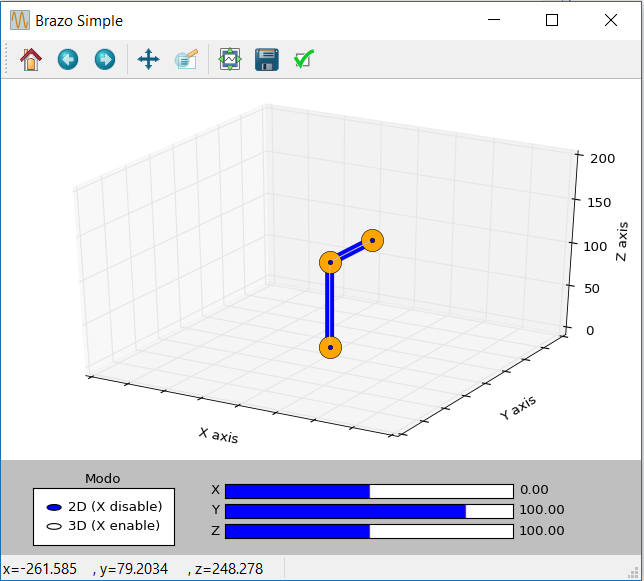
\includegraphics[scale=0.85]{imagenes/disenio_ventana}

Empezaremos creando la ventana(fig) con un nombre, y dentro de ella la ventana de dibujado(ax) y el panel de error(axerror).

\lstinputlisting[language=Python,firstline=38,lastline=42]{codigos/brazo.py}

Ahora crearemos los widgets que vamos a usar que, como se ve en la imagen, son tres Sliders, uno por coordenada y un Radio Button para cambiar de Modo, dejaremos el Slider de la X desactivado ya que inicialmente el Modo será 2D y por tanto se moverá en el plano X=0.

\lstinputlisting[language=Python,firstline=43,lastline=60]{codigos/brazo.py}

Después añadimos los manejadores de eventos de los 4 widgets. Cuando el valor de alguno de los  Sliders se actualizará el valor de las variables de clase tx, ty o tz, según de cual se haya modificado el valor, y se llamará a la función draw\_robot, la cuál veremos más adelante.
En el caso del manejador del Radio Button del Modo, este activará o desactivará el Slider X y cambiará la variable de clase modo.

\lstinputlisting[language=Python,firstline=62,lastline=90]{codigos/brazo.py}

Ya solo nos queda llamar a display\_error, a drow\_robot y hacemos show para dibujarlo todo.

\lstinputlisting[language=Python,firstline=91,lastline=95]{codigos/brazo.py}

Y con esto habríamos terminado el constructor, Ahora escribimos algunas funciones de la clase, empezando por preparar una señal de error que nos indicara cuando se le a solicitado al brazo acceder a una posición fuera de su alcance.

\lstinputlisting[language=Python,firstline=97,lastline=104]{codigos/brazo.py}

La función siguiente es la encargada de, usando todo lo preparado en el constructor y los valores introducidos por los Sliders, obtener los valores de c1,s1,c2,s2 y una vez comprobado que son números reales, si son imaginarios activamos el display\_error, actualizar los valores de y[1] y z[1]. Para hacer esto usaremos, de los dos valores posibles de s1, el positivo para así evitar problemas al cambiar de cuadrante.
También situaremos y[2] y z[2] en la posición elegida en los Sliders.

Tanto x[1], como x[2] serán puestas a 0 ya que esta función es para el modo 2D.

\lstinputlisting[language=Python,firstline=105,lastline=132]{codigos/brazo.py}

Para el caso en 3D vamos a usar un cambio a coordenadas esféricas, esto es:
\[
\left \{
\begin{array}{lll}
x = r\cdot sin(\theta)\cdot cos(\varphi)\\
y = r\cdot sin(\theta)\cdot sin(\varphi)\\
z = r\cdot(\varphi)
\end{array}
\right .
\left .
,\;siendo\; \varphi
\right .
=
\left \{
\begin{array}{lll}
arctan\left(\frac{y}{x}\right) 			& x>0\; y\; y>0\\
2\pi + arctan\left(\frac{y}{x}\right)	& x>0\; y\; y<0\\
\frac{\pi}{2}\cdot sgn(y)						& x=0\\
\pi + arctan\left(\frac{y}{x}\right) 	& x<0\\
\end{array}
\right .
\]


\lstinputlisting[language=Python,firstline=133,lastline=172]{codigos/brazo.py}

A continuación vemos las funciones set\_positions y set\_ax.
La primera será la que dibuje el robot, y la segunda la que dibuje el sistema de coordenadas.

\lstinputlisting[language=Python,firstline=173,lastline=193]{codigos/brazo.py}

Por último tenemos la función draw\_robot la cual tendrá en cuenta el modo para calcular Gröbner en 2D o en 3D y, tras estos cálculos, ver si estamos ante un estado posible o no. Si el estado es posible no dibujaremos la señal de error y dibujaremos tanto los ejes como el brazo y en caso contrario, solo dibujaremos el error.
Por ultimo hacemos draw para dibujar todo. 

\lstinputlisting[language=Python,firstline=194,lastline=207]{codigos/brazo.py}

Y ya fuera de la clase, tenemos el main que lo único que hace es crear un objeto Draw\_robot. 

\lstinputlisting[language=Python,firstline=209,lastline=250]{codigos/brazo.py}

%
%\input{capitulos/06_Implementacion}
%
%\input{capitulos/07_Pruebas}
%
%\input{capitulos/08_Conclusiones}
%
%%\chapter{Conclusiones y Trabajos Futuros}
%
%
%%\nocite{*}
%\bibliography{bibliografia/bibliografia}\addcontentsline{toc}{chapter}{Bibliografía}
%\bibliographystyle{miunsrturl}
%
%\appendix
%\input{apendices/manual_usuario/manual_usuario}
%%\input{apendices/paper/paper}
%\input{glosario/entradas_glosario}
% \addcontentsline{toc}{chapter}{Glosario}
% \printglossary
\chapter*{}
\thispagestyle{empty}

\end{document}
